\chapter{VLSI Design}
First of all, what is VLSI?\\
\begin{boxH}
  \textbf{VLSI} stands for \textit{Very Large Scale Integration}, and it is the process of creating an 
  Integrated Circuit (IC) by combining thousands of transistors into a single chip, which will
  be produced in a very large scale.
\end{boxH}
With VLSI design, we create a chip that:
\begin{itemize}
  \item has a complex design
  \item has a large digital part
  \item will be produces in a large scale
\end{itemize}
As the technology progresses, the number of transistors that can be put into a single chip
has largely increased, which means that the design of the chip has become more complex, and cannot 
be done by hand anymore.\\
For this reason we need to use a tool that can help us design the chip, that allow us to design 
by drawing rectangles and lines, and then the tool will take care of the rest.
\begin{section}{VLSI design flow}
  The design flow is structured in different levels of abstraction, as shown in figure \ref{fig:vlsi design flow}.\\
  The first level is the \textbf{system level}, where we define the functionality of the chip, 
  which are provided by different \textbf{modules}. Each module can be represented by gates, which 
  are just a combination of digital circuits, which are made up of transistors.\\
  \begin{figure}[H]
    \centering
    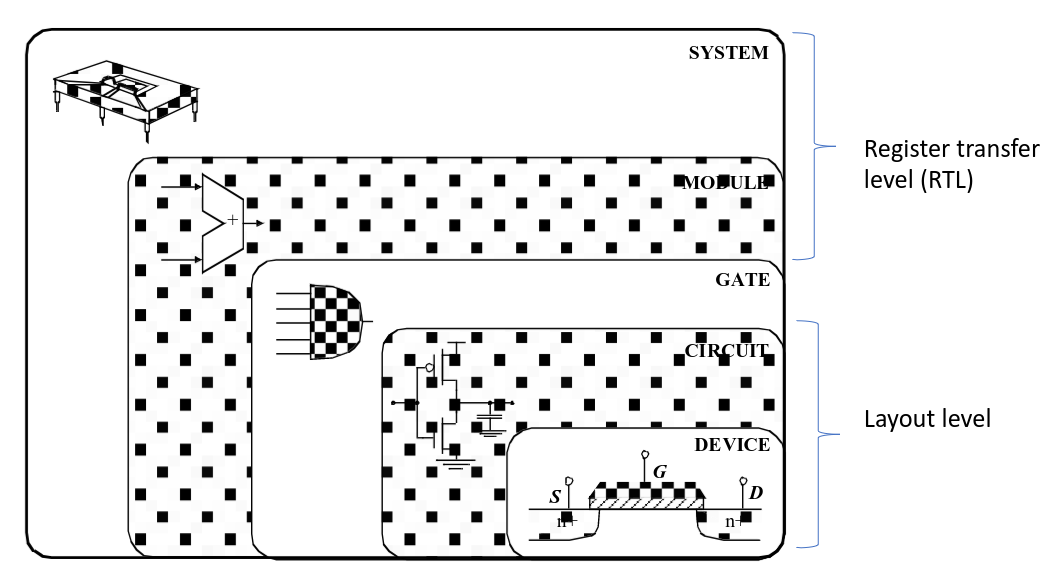
\includegraphics[width=0.7\textwidth]{img/hardware/vlsi design flow16.png}
    \caption{VLSI design flow}
    \label{fig:vlsi design flow}
  \end{figure}
  \begin{subsection}{Device}
    Nowadays, most of the devices (at least 90\% according to Maurizio Martina) are Metal-Oxide 
    Semiconductor Field-Effect Transistors (MOS transistors).\\
    Those transistors are a 4 terminal device made up of a \textbf{source}, a \textbf{drain} and a 
    \textbf{gate}, as you can see in figure \ref{fig:transistor}, and rely on a layer of a 
    semiconductor, which is almost always Silicon, called \textbf{bulk}.\\
    On top of the bulk, there's a layer of insulator and one of metal(usually).
    \begin{figure}[H]
      \centering
      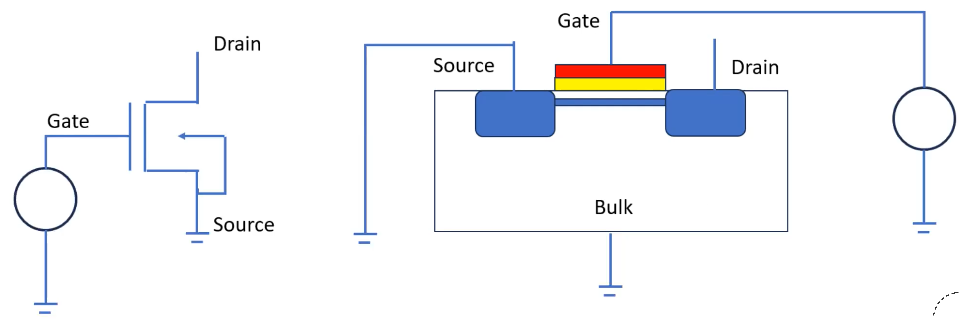
\includegraphics[width=0.6\textwidth]{img/hardware/transistor.png}
      \caption{Logical structure of a transistor}
      \label{fig:transistor}
    \end{figure}
    A transistor is nothing more than a switch, that can be open or closed, depending on the
    voltage applied to the gate, making the current flow from the source to the drain.\\
    As you think of it, it works like a water flow, where the gate is the valve, the source is the
    water source and the drain is the sink. This works if we have some pressure, that is the voltage
    applied to the gate, causing a difference of voltage between the source and the drain.\\
    So, by applying a voltage to the gate, we can open it, but because we need a difference of
    voltage between the source and the drain, we need to apply a voltage to the drain and connect 
    the source to the ground.\\
    The amount of current that can flow from the source to the drain is 
    \begin{equation}
      I_{DS} = f(V_{GS}, V_{DS})
    \end{equation}
    where $I_{DS}$ is the current flowing from the source to the drain, $V_{GS}$ is the voltage
    difference between the gate and the source, which modulates the width of the channel, and 
    $V_{DS}$ is the voltage difference between the drain and the source.\\
    But if we have a current which is a function of a voltage, we can also have a resistance, because
    the resistance is the ratio between the voltage and the current, and the Hall law states that
    a current is proportional to the voltage and inversely proportional to the resistance.\\
    Furthermore, the channel resistance depends also on a geometric factor, which is the length and
    the width of a channel:
    \begin{equation}
      R_{ch} \varpropto \frac{L}{W} \to I_{DS}  \varpropto \frac{V_{DS}}{R_{ch}}\to I_{DS} \varpropto \frac{W}{L} V_{DS}
      \label{eq:channel resistance}
    \end{equation}
    Equation \ref{eq:channel resistance} shows that the amount of current flowing in the transistor
    is proportional to this geometric factor. This is because the current flowing is inversely
    proportional to the resistance, meaning that the current increases with the width of the channel
    and decreases with the length of the same.\\
    Hall law also says that the material of the channel has an impact, but we will not consider it.\\

    We can also quantify how much current is flowing in the transistor by using the following
    equation:
    \begin{equation}
      I_{DS} = \mu C_{ox} \frac{W}{L} [(V_{GS} - V_{TH}) V_{DS} - \frac{V_{DS}^2}{2}]
      \label{eq:current}
    \end{equation}
    where:
    \begin{itemize}
      \item $\mu$ is the mobility of the charge carriers
      \item $C_{ox}$ is the capacitance of the oxide layer
      \item $V_{TH}$ is the threshold voltage
      \item $W$ is the width of the channel
      \item $L$ is the length of the channel
      \item $V_{GS}$ is the voltage difference between the gate and the source
      \item $V_{DS}$ is the voltage difference between the drain and the source
    \end{itemize}
    Thankfully we are not proving that, but the first three terms are tied to the technology, while 
    with the others we can modulate the current flowing in the transistor.
    \begin{subsubsection}{Saturation}
      Experimental result shows that, if we have no voltage we have no current, and if we increase
      the drain to source voltage, the current increases. But if we increase the voltage too much, 
      the current will not increase anymore, remaining constant, and this is called 
      \textbf{saturation}.\\
      This also means that the current is no longer proportional to the voltage, but if we can generate
      a current independent from the voltage, meaning that on certain conditions a transistor can be
      an ideal current generator.\\
      Furthermore, the saturation point depends on:
      \begin{itemize}
        \item the technology
        \item the geometry of the transistor
        \item the square of the voltage difference between the gate and the source
      \end{itemize}
      and can be described as:
      \begin{equation}
        I_{DSS} = \frac{\mu C_{ox}}{2} \frac{W}{L} (V_{GS} - V_{TH})^2
        \label{eq:saturation}
      \end{equation}
      \begin{figure}[h]
        \centering
        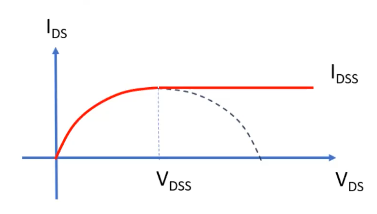
\includegraphics[width=0.5\textwidth]{img/hardware/saturation.png}
        \caption{Graphical representation of the saturation point $I_{DSS}$ of  a transistor}
        \label{fig:saturation}
      \end{figure}
      An additional observation that we can do is that the growth of the current is not linear, and 
      also very steep, meaning that a transistor can act as a very good amplifier.\\
    \end{subsubsection}
    \begin{subsubsection}{Digital circuits}
      Digital electronics is much simpler than analog electronics, because we have only two states:
      0 and 1.\\
      This can be transposed to the voltage, where we can observe that:
      \begin{itemize}
        \item if there's no voltage between the gate and the source($V_{GS}$), the transistor is off,
          meaning there's no current flowing($I_{DS} = 0$)
        \item if there's voltage between the gate and the source, but the voltage between the drain
          and the source is 0($V_{DS} = 0$), no difference of voltage means no current flowing
          ($I_{DS} \approx 0$)
        \item if both $V_{GS}$ and $V_{DS}$ are different from 0, the transistor is on and 
          in saturation, meaning that the current is flowing($I_{DS} = I_{DSS}$)
      \end{itemize}
      All this also depends on the width and the length of the MOS transistor.
    \end{subsubsection}


  \end{subsection}
  \begin{subsection}{Transistor types}
    Actually, the transistor described in the previous section is a \textbf{NMOS} transistor, which
    composing material are described in figure \ref{fig:nmos transistor}.
    \begin{figure}[h]
      \centering
      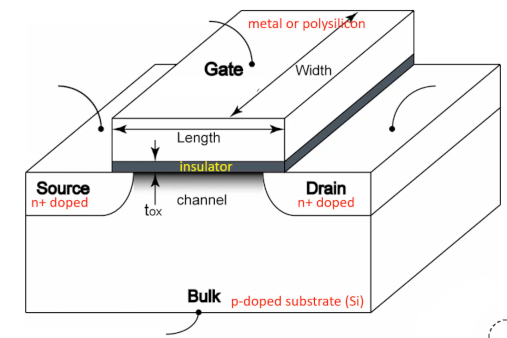
\includegraphics[width=0.5\textwidth]{img/hardware/nmos tranistor.png}
      \caption{Composing material of a NMOS transistor}
      \label{fig:nmos transistor}
    \end{figure}
    \begin{subsubsection}{Building up a NMOS transistor}
      As previously said, designing a transistor means drawing rectangles and lines.
      First of all, we have to draw the n-region, which is the boundary of the transistor, and then
      we can place the gate, which defines the width and the length of the transistor.\\
      After that, we can draw the source and the drain, which are the terminals of the transistor, 
      and their metal contacts.\\
      The last step is to add a further terminal which provide voltage to the bulk.
      \begin{figure}[h]
        \centering
        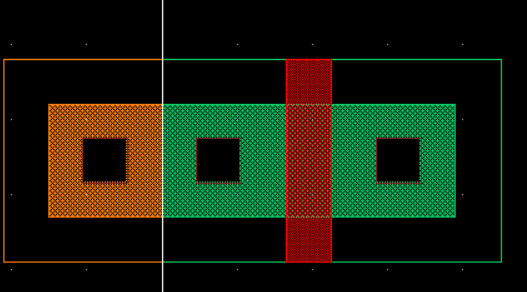
\includegraphics[width=0.5\textwidth]{img/hardware/nmos design.png}
        \caption{Possible design of a NMOS transistor, in red the gate, in green the source and drain
        terminals and in orange the bulk terminal}
        \label{fig:nmos transistor design}
      \end{figure}
      The surface of the component cannot be arbitrary but depends on the technology(or design 
      rules, a set or rules about the geometry).
    \end{subsubsection}
    \begin{subsubsection}{pMOS transistors}
      The pMOS transistor is the opposite of the NMOS transistor, and is made up of p-type material,
      on top of a n-type well.\\
      The design is the same, but the source and the drain are connected to the voltage source, and
      the gate is connected to the ground.\\
      The bulk terminal is connected to the source and the drain, and the gate is connected to the 
      ground.
      \begin{figure}[h]
        \centering
        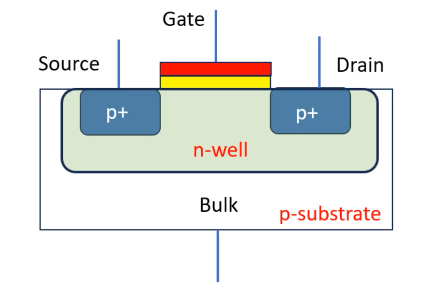
\includegraphics[width=0.5\textwidth]{img/hardware/pmos transistor.png}
        \caption{Structure of a pMOS transistor}
        \label{fig:pmos transistor}
      \end{figure}
      The main difference between the two transistors is that the p-type NMOS transistor transports
      holes, while the n-type NMOS transistor transports electrons. Holes are just electrons with
      positive charge, as a simple way to think about it. Because it is complementary to the NMOS
      transistor, when the difference of voltage between the gate and the source greater than the
      threshold voltage, the transistor is off, having no current flowing.\\
      When the voltage is less than the threshold voltage, the transistor is on, and the current is
      negative, meaning that the current is flowing from the source to the drain, or in formal terms
      :
      \begin{equation}
        I_{DS} = \begin{cases}
          0 & \text{if } V_{GS} > V_{TH}\\
          < 0 & \text{if } V_{GS} < V_{TH}
        \end{cases}
      \end{equation}
      This behaviour is troublesome from a physical point of view, because the current is negative,
      so to solve it we can invert the current, and to do so we need a voltage difference between the
      source and the gate, which allows the current to flow from the source to the drain.
      \begin{boxH}
        So to sum up the behaviour of the pMOS transistor:
        \begin{itemize}
          \item it needs a negative voltage between the gate and the source to be on
          \item the current flows from source to drain
        \end{itemize}
      \end{boxH}
    \end{subsubsection}
    \begin{subsubsection}{CMOS inverter}
      The CMOS technology is the combination of the NMOS and the pMOS transistors. It actually behaves
      like an inverter, because the output is the opposite of the input.\\

      \begin{figure}[h]
        \centering
        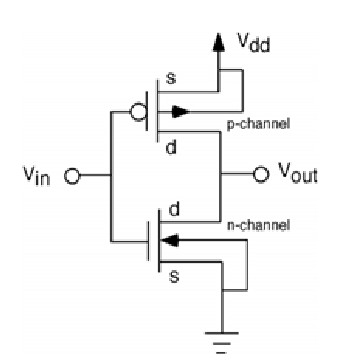
\includegraphics[width=0.3\textwidth]{img/hardware/cmos inverter.png}
        \caption{An example of a CMOS inverter}
        \label{fig:cmos inverter}
      \end{figure}
      Here's an interesting observation about this inverter: if the input is 0, the NMOS transistor
      is off, and the pMOS transistor is on, meaning that the voltage between the nMOS and the output
      is 0, but for Kerckhoff's law, the voltage between the pMOS and the output is 0 too, because 
      the sum of the current at the output node must be 0, even though the pMOS is on.\\
      But as for the Hall law, the current is proportional to the voltage, so no current means no
      voltage, if we have no voltage drop, the voltage of the output is exactly the same as the
      pMOS, which is actually the voltage of the power supply($V_{out}=V_{dd}$).\\
    \end{subsubsection}
    \begin{subsubsection}{Other logic functions}
      We can observe that by combining the NMOS and the pMOS transistors we can create other logic
      functions, like the AND, OR and XOR functions.\\
      For example it is possible to build a NAND gate by combining a NMOS and a pMOS transistor.
      \begin{figure}[h]
        \centering
        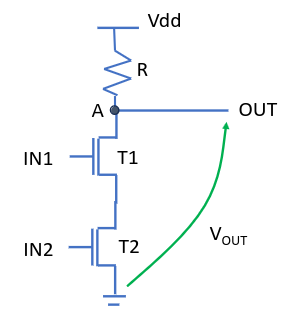
\includegraphics[width=0.3\textwidth]{img/hardware/nand gate.png}
        \caption{An example of a NAND gate}
        \label{fig:nand gate}
      \end{figure}
      We are actually able to build any combination function, it is just a matter of increasing the
      complexity of the circuit.\\
    \end{subsubsection}
  \end{subsection}
\end{section}
